\documentclass[border=10pt]{standalone}
\usepackage{pgfplots}
\usepackage{xcolor}
\pgfplotsset{width=7cm,compat=1.8}
\newcommand{\drawStackedBarPlots}{%
\addplot+[ybar, fill=blue!80!black, draw=teal!90!black, line width=1.2pt] 
    coordinates {(itemA,1) (itemB,3) (itemC,0) (itemD,2) (itemE,2) (itemF,1) (itemG,2)};
\addplot+[ybar, fill=teal!80!black, draw=blue!80!black, line width=1.2pt] 
    coordinates {(itemA,0) (itemB,2) (itemC,1) (itemD,1) (itemE,0) (itemF,2) (itemG,0)};
\addplot+[ybar, fill=gray!70!black, draw=teal!70!black, line width=1.2pt] 
    coordinates {(itemA,5) (itemB,4) (itemC,7) (itemD,3) (itemE,5) (itemF,4) (itemG,5)};
\addplot+[ybar, fill=cyan!70!black, draw=blue!70!black, line width=1.2pt] 
    coordinates {(itemA,3) (itemB,1) (itemC,2) (itemD,4) (itemE,1) (itemF,3) (itemG,3)};
\legend{\strut absent, \strut seldom, \strut regular, \strut frequent}%
}
\begin{document}
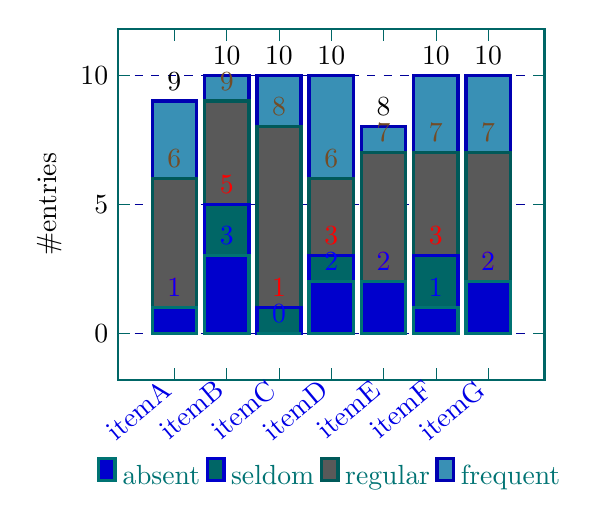
\begin{tikzpicture}
\begin{axis}[
    ybar stacked,
    bar width=16pt,
    nodes near coords,
    enlargelimits=0.18,
    legend style={
        at={(0.5,-0.20)},
        anchor=north,
        legend columns=-1,
        draw=none,
        fill=none,
        text=teal!90!black
    },
    ylabel={\#entries},
    symbolic x coords={itemA, itemB, itemC, itemD, itemE, itemF, itemG},
    xtick=data,
    x tick label style={rotate=40,anchor=east, text=blue!90!black},
    axis line style={thick, color=teal!80!black},
    tick style={color=teal!80!black},
    ymajorgrids=true,
    grid style={dashed, color=blue!60!black},
]
\drawStackedBarPlots
\end{axis}
\end{tikzpicture}
\end{document}
